\documentclass[12pt]{article}
\usepackage[utf8]{inputenc}
\usepackage[left=2.5cm, right=2.5cm, top=2.0cm]{geometry}
\usepackage{sectsty}
\usepackage{graphicx}
\usepackage{amsmath}
\usepackage{amssymb}
\usepackage{undertilde}
\usepackage{kbordermatrix}
\usepackage{listings}
\usepackage{ulem}
\usepackage{soul}
% \usepackage{tikz}
% \usepackage{pgfplots}
% \pgfplotsset{compat=1.16} 
\usepackage{siunitx}
\usepackage{pythonhighlight}
\usepackage{caption}
\usepackage{float}
\usepackage{url}
\usepackage{enumitem}
\usepackage{bm}
\usepackage{empheq}
\usepackage{tcolorbox}
\usepackage{framed}
\usepackage{xparse}
\usepackage{algorithm, algorithmic}
% \usepackage{algorithmic}
\usepackage{booktabs}
\usepackage{tabularx}
\usepackage{hyperref}
\usepackage{mathtools}
\DeclareMathOperator*{\argmax}{arg\,max}
% \usepackage[shortlabels]{enumitem}
\tcbuselibrary{breakable}


%  ---------------------- COMMANDS ---------------------------
% Double underline
\def\dunderline#1{\underline{\underline{#1}}}

% Shorten nonumber command
\def\nnb{\nonumber}

% Shorten boldsymbol command
\def\bs#1{\boldsymbol{#1}}

% Algorithmic newline
\def\algonewline{\STATE{ }}

% Eigenvectors of
\def\eigvecof{\text{eigenvectors of }}

% Eigenvalues of 
\def\eigvalof{\text{eigenvalues of }}

% Enclose in square brackets
\newcommand{\enclb}[1]{\left[#1\right]}
% Enclose in parenthesis
\newcommand{\enclp}[1]{\left(#1\right)}
% Enclose in curly brackets
\newcommand{\enclc}[1]{\left\{#1\right\}}

% Annotate first argument, text in second argument
\newcommand{\overtext}[2]{\overbrace{#1}^{\mathclap{\text{#2}}}}
\newcommand{\undertext}[2]{\underbrace{#1}_{\mathclap{\text{#2}}}}

% Normalization constant in multivariate normal
\newcommand{\mvnconst}[1]{\frac{1}{(2\pi)^{d/2} |#1|^{1/2}}}

% Exponential factor in multivariate normal
\newcommand{\mvnexpo}[3][x]{\exp \left[  -{\frac{1}{2}} (#1 - #2)^T #3^{-1} (#1 - #2) \right]}

% Multivariate normal
\newcommand{\mvn}[3][x]{\mvnconst{#3} \mvnexpo[#1]{#2}{#3}}

% For numbering in align* environment
\newcommand{\numberthis}{\addtocounter{equation}{1}\tag{\theequation}}

%  Sum notation w/ limits as argument and index as option
\newcommand{\sumlim}[3][i]{\sum\limits_{#1=#2}^{#3}}

%  Product notation w/ limits as argument and index as option
\newcommand{\prodlim}[3][i]{\prod\limits_{#1=#2}^{#3}}

%  Sum notation with only information beneath
\newcommand{\sumnolim}[1]{\sum\limits_{#1}}

%  Integral notation w/ limits as argument and index as option
\newcommand{\intlim}[2]{\int\limits_{#1}^{#2}}

%  Integral over whole domain notation, no args
\newcommand{\intinf}{\int\limits_{-\infty}^{\infty}}

%  Partial derivative notation, arg1: numerator, arg2: denominator
\newcommand{\pfrac}[3][ ]{\frac{\partial^{#1} #2}{\partial #3^{#1}}}

%  Derivative notation, arg1: numerator, arg2: denominator
\newcommand{\dvfrac}[3][ ]{\frac{\text{d}^{#1} #2}{\text{d} #3^{#1}}}

% When doing Gauss-Jordan, create arrow showing operations
\newcommand{\ro}[1]{\xrightarrow{\mathmakebox[\rowidth]{#1}}}

% ----------------------INVIRONMENTS---------------------------
% Item list with title
\newenvironment{titlemize}[1]{%
  \paragraph{#1}
  \begin{itemize}}
  {\end{itemize}}

  % Enum list with title
\newenvironment{titleenum}[1]{%
  \paragraph{#1}
  \begin{enumerate}}
  {\end{enumerate}}

  % Augmented matrix (matrix with vertical line)
\newenvironment{sysmatrix}[1]
  {\left(\begin{array}{@{}#1@{}}}
  {\end{array}\right)}

 % Make matrices with more spacing
\makeatletter
\renewcommand*\env@matrix[1][\arraystretch]{%
  \edef\arraystretch{#1}%
  \hskip -\arraycolsep
  \let\@ifnextchar\new@ifnextchar
  \array{*\c@MaxMatrixCols c}}
\makeatother

% \renewcommand*{\arraystretch}{1.5}

\newlength{\rowidth}% row operation width
\AtBeginDocument{\setlength{\rowidth}{3em}}

\floatname{algorithm}{Algorithm}
\renewcommand{\algorithmicrequire}{\textbf{Input:}}
\renewcommand{\algorithmicensure}{\textbf{Output:}}

\begin{document}
\title{\textbf{INF367A Exercise 8}}
\author{Naphat Amundsen}
\maketitle
\sectionfont{\fontsize{14}{15}\selectfont}
\subsectionfont{\fontsize{12}{15}\selectfont}
\subsubsectionfont{\fontsize{12}{15}\selectfont}
\graphicspath{ {./images/} }

\ifx
\begin{figure}[H]
	\centering
	\includegraphics[scale=0.8]{Figure_2}
	\caption{Insert caption here}
\end{figure}
\fi

\section*{Introduction}
    This exercise is about using the Expectation-Maximization algorithm on Gaussian Mixture Models.

\section{EM algorithm for GMMs}
    \begin{tcolorbox}[breakable]
        In this exercise, we try to find clusters of large cities. Download the data set largest\_cities.csv which contains the coordinates (longitude and latitude) of the 500 largest cities in the world. 
        
        \begin{enumerate}
            \item Implement the EM algorithm for GMMs using the formulas in the lecture slides 
            \item Compute log-likelihood $\log P(x|\theta) = \sumlim{1}{n} \log \enclb{\sumlim[k]{1}{K}\pi_k N(x_i|\mu_k, |\Sigma_k)}$ after each M-step. Sanity check: log-likelihood should increase after each step 
            \item Use BIC to choose the number of components $K$. Note that representing one d-dimensional component requires $d+(d+1) \times d/2$ parameters ($d$ parameters for the mean vector and $(d+1) \times d/2$ parameters for the covariance matrix). In addition, we need $K-1$ parameters for mixing coefficients (-1 is there because mixing coefficients sum to one). Thus, the total number of parameters is $K \times (d + (d + 1)d/2) + (K - 1).$ 
        \end{enumerate}
        
        Hints: The EM algorithm is sensitive to initialization. Therefore, you may want to try several different initializations. You may encounter 
        \begin{verbatim}
            ValueError: array must not contain infs or NaNs
        \end{verbatim}
        because some responsibilities are \verb|nan|. This is typically due to some data points lying so far away from all the cluster centers that Python interprets all probabilities as $0$. In this case, you should try to initialize covariance matrices with larger variances.

    \end{tcolorbox}

    \subsection{Implementing the EM-algorithm for a GMM}
        The EM algorithm consists of two steps: Expectation and Maximization. Where the Expectation step (E-step) calculates the probability $\pi_{ij}$ of a data point $\bs x_i$ coming from each component $C_j$, i.e 

        \begin{empheq}[box=\fbox]{align}
            \pi_{ij} = P(C_j | \bs x_i) \label{pi}
        \end{empheq}

        The Maximization step (M-step) then assumes that each $\pi_{ij}$ (also called weights) are correct, and then updates the parameters for the components which are modelled by the Multivariate Gaussians $\mathcal{N}_c(\bs \mu_c,\,\bm\Sigma_c, \Phi_c)$. The formulas used to update the parameters are essentially the "weighted" versions of the MLEs for the case of known labels:

        \begin{empheq}[box=\fbox]{align}
            \hat{\bs \mu_j} &= \frac{\sum\limits_{i=1}^{N} w_{ij} \bs x_i}{\sum\limits_{i=1}^{N} w_{ij}} \label{mu}
        \end{empheq}

        \begin{empheq}[box=\fbox]{align}
            \hat{\bm \Sigma_j} &= \frac{\sum\limits_{i=1}^{N} w_{ij} (\bs x_i - \bs \mu) (\bs x_i - \bs \mu)^T}{\sum\limits_{i=1}^{N} w_{ij}} \label{sigma}
        \end{empheq}

        Where the mixing probabilities are
        \begin{empheq}[box=\fbox]{align}
            \hat{\Phi_j} &= \frac{\sum\limits_{i=1}^{N} w_{ij}}{N} \label{phi}
        \end{empheq}

        It should also be noted that one initializes the algorithm with arbitrary values for the parameters.

    \subsection{Design}
        \begin{titlemize}{Parameters}
            \item N = Number of data points 
            \item k = Number of components / predicted clusters
        \end{titlemize}

        In the initialization phase, the program creates array \textbf W of size $(N \times k)$ as a container for each data-weight $\pi_{ij}$. Each column in the array is respective to each component. Each component are defined by their respective sets of variables, which are also stored in arrays. 

        \begin{titleenum}{E-step}
            \item Calculate the data weights for each component using (\ref{pi}) and store them in \textbf W
            \item Divide each row of \textbf W by the sum of the same row of itself. 
        \end{titleenum}
        

        \begin{titleenum}{M-step}
            \item For each component do:
            \begin{enumerate}
                \item Update the mean using (\ref{mu})
                \item Update the covariance matrix using (\ref{sigma}) 
                \item Update the mixing probability using (\ref{phi})
            \end{enumerate}
        \end{titleenum}

    The E and M steps are repeated until either a maximum number of iterations are reached or the likelihood  changes with a sufficiently low delta between iterations.

    \begin{table}[H]
        \centering
        \caption{Using the EM-Algorithm with number of components between 2 and 18 with yielded the following table. To accommodate the sensitivity to starting parameters, the EM algorithm is ran six times, of which gives us multiple columns for BICs. Bolded elements indicates best performances.}
        \begin{tabular}{lrrrrrr}
            \toprule
                models &    BIC\_1 &    BIC\_2 &    BIC\_3 &    BIC\_4 &    BIC\_5 &    BIC\_6 \\
            \midrule
            GMM(k=2) & -5000.13 & -4952.60 & -5000.13 & -4952.60 & -5000.13 & -5000.13 \\
            GMM(k=3) & -4863.11 & -4859.00 & -4948.97 & -4859.00 & -4920.91 & -4948.97 \\
            GMM(k=4) & -4864.77 & -4820.61 & -4820.61 & -4820.61 & -4809.86 & -4809.86 \\
            GMM(k=5) & -4816.59 & -4806.08 & -4780.18 & -4794.38 & -4794.38 & -4814.87 \\
            GMM(k=6) & -4799.90 & -4779.96 & -4795.46 & -4768.47 & -4801.31 & -4786.50 \\
            GMM(k=7) & -4772.40 & -4750.28 & -4765.29 & -4791.78 & -4773.76 & -4797.49 \\
            GMM(k=8) & -4790.45 & -4761.65 & -4766.06 & -4774.73 & -4767.99 & -4806.17 \\
            GMM(k=9) & -4768.56 & -4781.17 & -4758.29 & -4810.91 & -4793.60 & -4746.56 \\
            \textbf{GMM(k=10)} & -4753.43 & \textbf{-4734.07} & -4798.40 & -4776.24 & -4796.92 & -4778.69 \\
            GMM(k=11) & -4770.90 & -4763.49 & -4762.60 & -4737.75 & -4777.17 & -4744.58 \\
            GMM(k=12) & -4781.50 & -4765.72 & -4761.48 & -4743.37 & -4784.90 & -4796.56 \\
            GMM(k=13) & -4742.97 & -4765.77 & -4748.39 & -4771.71 & -4759.71 & -4768.28 \\
            GMM(k=14) & -4769.40 & -4755.35 & -4757.60 & -4748.50 & -4743.99 & -4781.08 \\
            GMM(k=15) & -4790.03 & -4763.56 & -4794.54 & -4786.38 & -4764.57 & -4759.05 \\
            GMM(k=16) & -4797.05 & -4785.86 & -4773.59 & -4774.39 & -4806.46 & -4786.34 \\
            GMM(k=17) & -4776.43 & -4797.44 & -4784.10 & -4780.90 & -4821.30 & -4806.14 \\
            GMM(k=18) & -4803.84 & -4789.69 & -4771.69 & -4806.42 & -4790.30 & -4784.86 \\
            \bottomrule
        \end{tabular}
    \end{table}

    \begin{figure}[H]
        \centering
        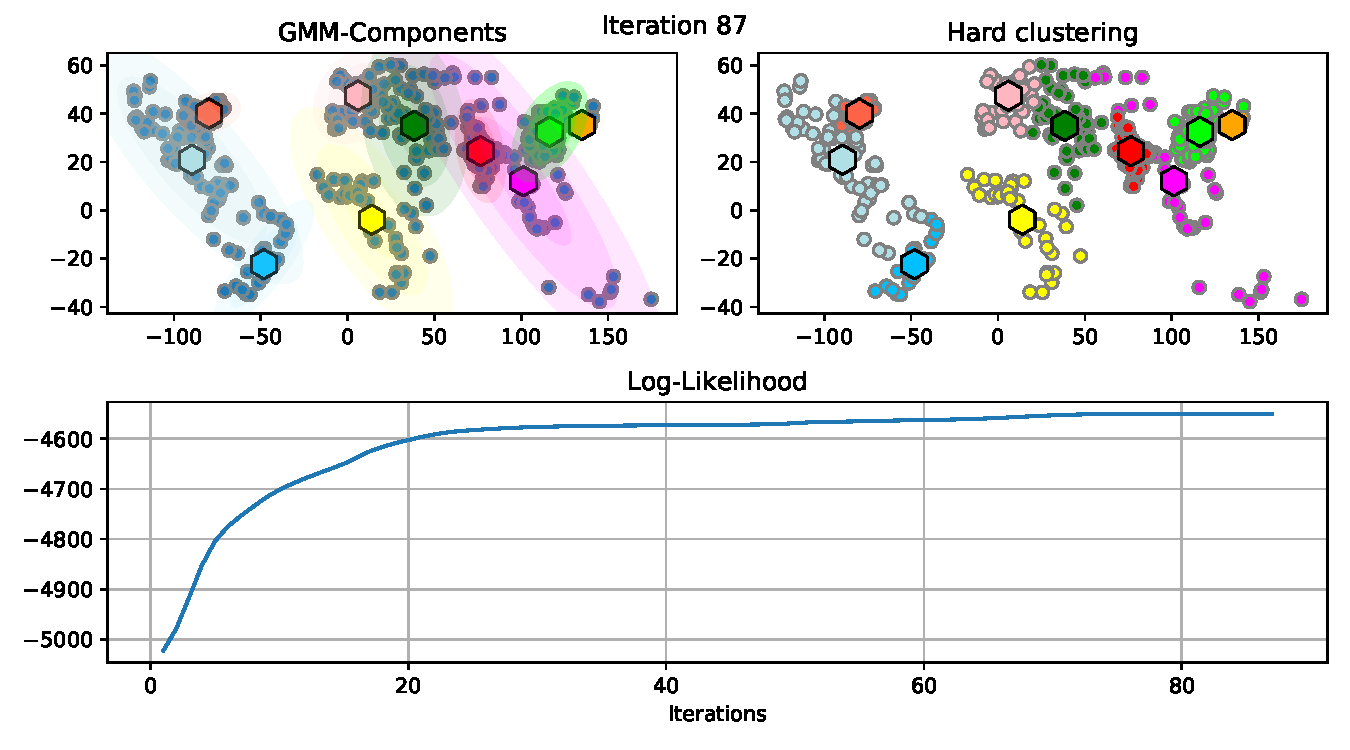
\includegraphics[width=0.95\textwidth]{GMM_task1.pdf}
        \caption{The output and log likelihood history of the best model. The upper left subplot visualizes the components. The opacity of the ellipses are linked to the mixing values.}
    \end{figure}

\section{Extension of the simple example}
    \begin{tcolorbox}[breakable]
        Suppose that we have $n$ independent observations $x = (x_1,\ldots,x_n )$ from a two-component mixture of univariate Gaussian distribution with unknown mixing coefficients and unknown mean of the second component: $P(x_i |\mu,p) = (1-p) \cdot N(x_i|0,1) + p \cdot N(x_i|\mu,1).$ 
        \begin{itemize}
            \item Write down the complete data log-likelihood and derive the EM-algorithm for learning maximum likelihood estimates for $\mu$ and $p$. 
            \item Implement the EM-algorithm. Load data ex8\_2.csv and learn the maximum likelihood estimates for $\hat{\mu}$ and $\hat{p}$. Plot the distribution $P(x_i| \hat{\mu}, \hat{p}).$ Does it match the observed data? Plot the log-likelihood of the observed data for each iteration (This should increase after each iteration) Hint: You can use simple\_example.pdf as a starting point.    
        \end{itemize}
    \end{tcolorbox}

    \def\zo{{z_{i1}}}
    \def\zt{{z_{i2}}}
    
    Ultimate goal is to maximize $\hat{\theta} = \argmax_\theta \log P(x|\theta)$. Let the variables $z={z_1, \ldots, z_i}$ denote the actual component responsible for generating observation $x_i$. In detail in the context of this task:
    \begin{align*}
        z_i = (\zo, \zt)^T = 
        \begin{cases}
            (1,0)^T, &\text{$x_i$ is from} \ N(x_i|0,1) \\
            (0,1)^T, &\text{$x_i$ is from} \ N(x_i|\mu,1)
        \end{cases}
    \end{align*}
    where we define the distributions for $z$ as follows:
    \begin{align*}
        P(\zo = 1) = (1-p) \\ 
        P(\zt = 1) = p  
    \end{align*}
    and
    \begin{align*}
        z_i = (\zo, \zt)^T = 
        \begin{cases}
            (1-p) \cdot N(x_i|0,1), &\text{if} \ \zo = 1\\
            p \cdot N(x_i|\mu,1), &\text{if} \ \zt = 1
        \end{cases}
    \end{align*}
    Then to obtain the probability of $x_i$ with respect to $\theta=(p, \mu)$, we can simply marginalize away $z$:
    \begin{align*}
        P(x_i|\theta) = \sumlim{1}{n} P(z_i) P(x_i|z_i, \theta)
    \end{align*}
    Then we can obtain the likelihood of the complete data $(x, z)$ (see lecture notes for definition):
    \begin{align}
        \log P(x,z|\theta) &= \log \enclb{\prodlim{1}{N} P(x_i, z_i|\theta)} = \sumlim{1}{n} \log P(x_i, z_i|\theta)\\
        &= \sumlim{1}{n} \log \enclb{P(z_i) N(x_i|0,1)^\zo N(x_i|\mu,1)^\zt} \\
        &= {\sumlim{1}{n} \log P(z_i) + \zo \log N(x_i|0,1) + \zt \log N(x_i|\mu,1)} \\ 
        &= \dunderline{\sumlim{1}{n} \log (\zo(1-p)+\zt p) + \zo \log N(x_i|0,1) + \zt \log N(x_i|\mu,1)}
    \end{align}

    \subsection*{E-step}
        First want to get expression for posterior distribution of latent variables given an estimate $\theta_t$ of $\theta$:
        \begin{align}
            P(\zo = 1|x_i, \hat{\theta_t}) &\propto P(\zo = 1) \overtext{P(\theta_t|\zo)}{$=1$} P(x_i|\theta_t,\zo) \\
            &= P(\zo = 1) P(x_i|\theta_t,\zo) \\
            &= (1-p) \cdot N(x_i|0,1)
        \end{align}
        \begin{align}
            P(\zt = 1|x_i, \hat{\theta_t}) &\propto P(\zt = 1) \overtext{P(\theta_t|\zt)}{$=1$} P(x_i|\theta_t,\zt) \\
            &= P(\zt = 1) P(x_i|\theta_t,\zt) \\
            &= p \cdot N(x_i|\mu,1)
        \end{align}
        Then by normalizing the values, we get the responsibilities / mixing probabilities:
        \begin{align}
            \gamma(\zo) &= \frac{(1-p) \cdot N(x_i|0,1)}{(1-p) \cdot N(x_i|0,1) + p \cdot N(x_i|\mu,1)} \\
            \gamma(\zt) &= \frac{p \cdot N(x_i|\mu,1)}{(1-p) \cdot N(x_i|0,1) + p \cdot N(x_i|\mu,1)} 
        \end{align}
        Note that $\gamma(\zo) + \gamma(\zt)=1$

        \vspace{5mm}
        \noindent The problem now is that $z_i$ is not observed. The solution is to maximize
        \begin{align}
            Q(\theta, \theta_t) &= E_{z|x_i,\theta_t} \enclb{\log P(x_i,z|\theta)} \\
            &= \sumlim{1}{n} E[\zo] \log N(x_i|0,1) + E[\zt] \log N(x_i|\mu,1) \\
            &= \sumlim{1}{n} \gamma(\zo) \log N(x_i|0,1) + \gamma(\zt) \log N(x_i|\mu,1) 
        \end{align}
        where $P(z|x,\theta_t)$ is the posterior distribution of the latent variables computed using the estimate $\theta_t$

    \subsection*{M-step}
        Maximize $Q(\theta, \theta_t)$ with respect to $\theta = (p, \mu)$. We maximize by setting derivative to zero. Note that 
        \begin{align*}
            \dvfrac{}{\mu} N(x_i|\mu, 1) = N(x_i|\mu,1)(x_i-\mu) 
        \end{align*}
        Simply differentiate with respect to each variable separately, lets start with respect to $\mu$ 
        \begin{align}
            \dvfrac{}{\mu} Q(\theta, \theta_t) &= \dvfrac{}{p} \sumlim{1}{n} (1-\gamma(\zt)) \log N(x_i|0,1) + \gamma(\zt) \log N(x_i|\mu,1) \\
            &= \sumlim{1}{n} \frac{\gamma(\zt)}{N(x_i|\mu,1)} N(x_i|\mu,1)(x_i-\mu) \\ 
            &= \sumlim{1}{n} \gamma(\zt)(x_i-\mu) = \sumlim{1}{n} \gamma(\zt)x_i - \gamma(\zt) \mu = 0 \\
            &\Rightarrow -\sumlim{1}{n} \gamma(\zt)\mu = -\sumlim{1}{n} \gamma(\zt)x_i \\
            &\Rightarrow \dunderline{\mu = \frac{\sumlim{1}{n} \gamma(\zt)x_i}{\sumlim{1}{n} \gamma(\zt)}} 
        \end{align}
        Then for $p$
        \begin{align*}
            \dvfrac{}{p} Q(\theta, \theta_t) &= \dvfrac{}{p} \sumlim{1}{n} (1-\gamma(\zt)) \log N(x_i|0,1) + \gamma(\zt) \log N(x_i|\mu,1)
        \end{align*}
        Recall that we actually have the constraint that $(1-p)+p = 1$. Since we have a constrained optimization problem, we use good ol' Lagrange optimization:
        \begin{align}
            \dvfrac{}{p} Q(\theta, \theta_t) &= \lambda \dvfrac{}{p} \enclb{(1-p)+p-1} = \lambda \dvfrac{}{p} 0 = 0 \\
            \dvfrac{}{p} Q(\theta, \theta_t) &= 0
        \end{align}
        Wolfram alpha says that 
        \begin{align*}
            \dvfrac{}{p} \gamma(\zt) &= \frac{N(x_i|0,1) \cdot N(x_i|\mu,1)}{(N(x_i|0,1)(1-p) - N(x_i|\mu, 1)p)^2} 
        \end{align*}
        Somehow from that we get (it's late, I am hungry now and want to just submit this)
        \begin{align}
            \dunderline{p = \frac{1}{n} \sumlim{1}{n} \gamma(\zt)}
        \end{align}

    \begin{figure}[H]
        \centering
        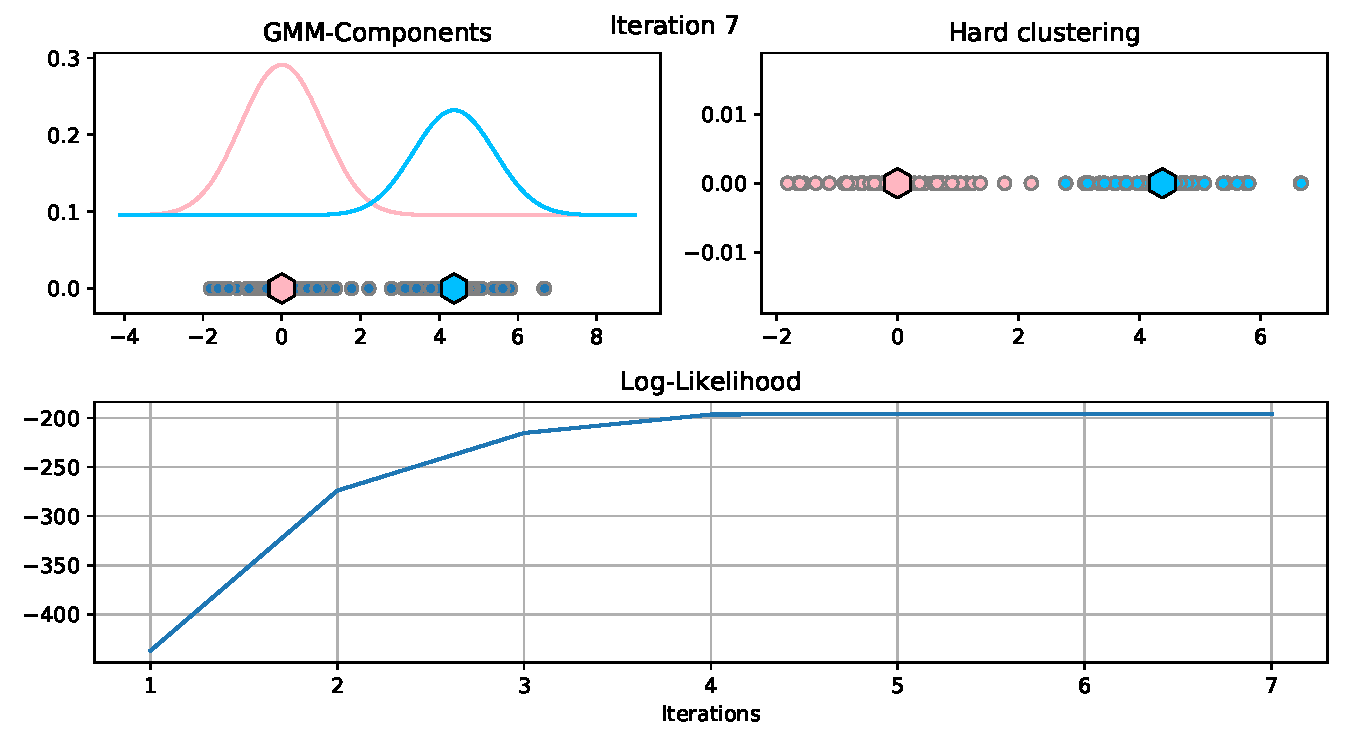
\includegraphics[width=0.95\textwidth]{GMM_task2.pdf}
        \caption{The output and log likelihood history of the best model. The upper left subplot visualizes the components. The opacity of the ellipses are linked to the mixing values.}
    \end{figure}
    The model seems to match the data well using the alternative EM algorithm.

    \appendix
    \section{GMM Class}
    \inputpython{EM_GMM.py}{0}{1000}
    \section{Rest of code}
    \inputpython{tasks.py}{0}{1000}

% \bibliographystyle{apalike}
% \bibliographystyle{ieeetran}
% \bibliography{citations}

\end{document}

